\chapter{Data and Knowledge Graph}
\label{chap:data-kg}

This chapter describes the data foundation used by the proposed question-answering system. The goal is to make clear what the True Demand knowledge graph contains, how it is represented, which parts of the graph are relevant for natural-language question answering, and where the limitations of the current data lie. This distinction is important because the reliability of a knowledge-graph question answering (KGQA) system depends not only on the LLM and the query-selection method, but also on the coverage, structure, and semantics of the underlying graph.

\section{True Demand Use Case}
\label{sec:true-demand-use-case}

The use case addressed in this thesis is natural-language question answering over the True Demand knowledge graph in the semiconductor supply-chain context. The True Demand concept is motivated by a practical business problem: demand signals in semiconductor supply chains are often uncertain, delayed, or distorted. Business partners may communicate requirements that do not directly correspond to actual demand, for example because of buffer-stock strategies, uncertainty about future production, or attempts to secure supply in constrained markets. Such behavior can amplify the bullwhip effect, where small changes in downstream demand propagate into larger fluctuations upstream in the supply chain.

The True Demand approach aims to move from assumption-based demand interpretation toward more structured, knowledge-based demand analysis. In the current graph, this is represented through survey-grounded data collected from different parts of the semiconductor and automotive ecosystem. The data captures reported demand, future-demand expectations, current-demand baselines, inventory trends, order-cancellation responses, shortage status, vehicle-sales observations, and autonomous-driving related indicators. These survey responses are represented as RDF triples and linked to common dimensions such as survey origin, region, quarter, vehicle type, technology category, component, and year.

From the perspective of this thesis, the business goal is not only to store the survey data, but to make it accessible to users who do not know SPARQL or the internal ontology structure. A business user should be able to ask questions such as:

\begin{itemize}
    \item ``Show total current demand from OEM customers by region.''
    \item ``How does future demand change by quarter and technology category?''
    \item ``What is the average autonomous-driving development percentage by vehicle type and SAE level?''
    \item ``How many companies report a shortage by survey type?''
\end{itemize}

These questions are simple at the user-interface level, but they require the system to identify the intended metric, select the correct graph class, determine grouping dimensions, generate or select a valid SPARQL query, execute it against the graph, and summarize the result. The True Demand use case is therefore well-suited for studying reliable LLM-based KGQA: the data is structured, the schema is non-trivial, and many user questions admit several plausible but semantically different query interpretations.

\subsection{Data provenance and transformation}
\label{subsec:data-provenance-transformation}

The data used in this thesis originates from structured True Demand survey artefacts rather than from unstructured web text. The survey process is designed to collect confidential demand-related signals from different actors in the semiconductor supply-chain ecosystem, including OEM, Tier1, and semiconductor-oriented perspectives. These inputs are transformed into a common RDF representation so that heterogeneous survey answers can be queried through a unified graph interface.

The transformation process maps survey fields and derived analytical outputs into typed RDF resources, predicates, and literal values. For example, company-related information is represented through company resources and survey-origin classes, regional demand records are represented through demand-analysis entities linked to regions, and time-related values are normalized into quarter, month, or year resources where supported by the data. Numeric survey values, such as demand quantities, percentage changes, participant counts, and vehicle-sales units, are represented as literal properties attached to the corresponding analysis or observation entities.

This provenance has two important consequences for the KGQA system. First, answers are graph-backed: a returned result must be supported by RDF triples produced from the survey transformation pipeline. Second, answerability is bounded by the actual survey coverage. A question may be meaningful from a business perspective but still not be answerable if the corresponding metric, dimension, or combination of dimensions was not collected or transformed into the graph. This is why the final system distinguishes between schema-valid questions and graph-supported questions.

\section{Graph Content}
\label{sec:graph-content}

The current True Demand RDF graph contains survey-grounded observations and derived analytical records. The graph is stored as Turtle and executed through SPARQL, either locally through RDFLib or through Apache Jena Fuseki. In the current exported version used for the experiments, the graph contains 1,159,883 RDF triples, 102,590 resource nodes, and 102,564 subject entities. The graph uses 85 distinct predicates at the RDF level. A companion schema abstraction is stored separately in JSON and contains 58 classes, 32 object-style predicates, 48 literal/data properties, and 70 declared relationships.

\begin{table}[ht]
\centering
\caption{Scale of the True Demand graph and schema used in this thesis.}
\label{tab:true-demand-scale}
\begin{tabular}{lr}
\hline
\textbf{Element} & \textbf{Count} \\
\hline
RDF triples in graph & 1,159,883 \\
Resource nodes / entities & 102,590 \\
Subject entities & 102,564 \\
Distinct RDF predicates in graph & 85 \\
Schema classes & 58 \\
Schema predicates & 32 \\
Schema data properties & 48 \\
Declared schema relationships & 70 \\
\hline
\end{tabular}
\end{table}

The graph is not a generic public-domain knowledge graph. It is a domain-specific, survey-grounded graph designed around the True Demand setting. Its content can be grouped into eight main areas, which are also the main capability groups used by the KGQA system:

\begin{enumerate}
    \item \textbf{Future demand}: expected future demand changes by region, quarter, vehicle type, technology category, and survey group.
    \item \textbf{Regional/current demand}: regional demand quantities and percentage changes, linked to survey origin and time-related dimensions.
    \item \textbf{Vehicle sales}: actual and forecast vehicle-sales observations, mainly organized by time period and vehicle-related information.
    \item \textbf{Shortage status}: company-level shortage indicators and counts by survey group or shortage status.
    \item \textbf{Autonomous driving}: autonomous-driving development indicators by vehicle type, SAE level, year, and survey origin.
    \item \textbf{Inventory}: inventory-development and target-indicator information by component, technology category, and trend.
    \item \textbf{Order cancellation}: order-cancellation responses and participant counts by technology category and response type.
    \item \textbf{Catalog lookup}: available companies, regions, technology categories, and quarter labels.
\end{enumerate}

Table~\ref{tab:domain-capabilities} summarizes the major question-answering domains and the dimensions supported by the current system. These domains are important because they define which questions can be answered deterministically through graph-supported templates and which questions require LLM-based candidate generation and ranking.

\begin{table}[ht]
\centering
\caption{Main graph-supported capability areas used by the KGQA system.}
\label{tab:domain-capabilities}
\begin{tabular}{p{3.2cm}p{7.8cm}p{3.2cm}}
\hline
\textbf{Capability} & \textbf{Supported dimensions} & \textbf{Typical aggregations} \\
\hline
Future demand & Region, quarter, vehicle type, technology category, survey group & AVG, SUM, COUNT, MAX, MIN \\
Regional demand & Region, quarter, survey group, vehicle type & SUM, AVG, COUNT, MAX, MIN \\
Vehicle sales & Month, year, vehicle type & SUM, AVG, COUNT \\
Shortage & Shortage status, survey group, technology category & COUNT \\
Autonomous driving & Vehicle type, SAE level, year, survey group & AVG, COUNT, MAX \\
Inventory & Component, technology category, trend & SUM, COUNT \\
Order cancellation & Technology category, response type & SUM, COUNT \\
Catalog lookup & Companies, regions, technology categories, quarter labels & COUNT / list \\
\hline
\end{tabular}
\end{table}

\subsection{Answerable query capabilities}
\label{subsec:answerable-query-capabilities}

For practical KGQA, the system does not treat the schema as a flat list of terms. Instead, it uses a capability-oriented view of the graph. A capability is a graph-supported combination of a metric, one or more dimensions, an aggregation, and a valid SPARQL path that returns data. This is stricter than ontology membership alone. For example, \texttt{Month} is a valid class in the graph, but it is not automatically a valid breakdown dimension for every demand-related metric. Similarly, \texttt{Region} is a valid dimension, but the correct path from a metric to region depends on the analytical class involved.

This distinction is important for both accuracy and usability. If the system suggests a query completion such as ``future demand by region'', then the graph should contain a supported path for future-demand records grouped by region. Conversely, suggestions that are only schema-valid but return no rows should not be presented as guided options to the user. The capability layer therefore acts as an intermediate representation between the raw graph and the natural-language interface.

\begin{table}[ht]
\centering
\caption{Examples of answerable graph capabilities used by the system.}
\label{tab:capability-examples}
\begin{tabular}{p{3.6cm}p{4.1cm}p{4.0cm}p{2.6cm}}
\hline
\textbf{User intent} & \textbf{Graph capability} & \textbf{Required graph elements} & \textbf{Typical output} \\
\hline
Future demand by region & Future-demand analysis grouped by region & \texttt{FutureDemandAnalysis}, region-related predicates, demand-change values & Grouped table \\
Vehicle sales by month & Vehicle-sales units grouped by month & \texttt{VehicleSalesObservation}, \texttt{Month}, \texttt{unitsSold} & Monthly totals \\
Shortage by survey status & Shortage counts by survey group or status & \texttt{Company}, shortage predicates, survey-origin information & Grouped counts \\
Autonomous driving by vehicle type and SAE level & Average development percentage by vehicle and SAE level & \texttt{AutonomousDrivingDevelopment}, vehicle type, SAE level, percentage values & Grouped averages \\
Inventory trend by component & Inventory records grouped by component or trend & Inventory-development classes, component and trend predicates & Grouped table \\
\hline
\end{tabular}
\end{table}

The capability inventory is also used to reduce unnecessary LLM usage. Frequent and unambiguous capability patterns can be routed directly to deterministic SPARQL templates. More ambiguous questions, or questions outside the known capability inventory, are passed to the LLM-based candidate-generation and ranking pipeline. This separation allows the system to answer simple graph-supported questions quickly while preserving the more flexible LLM pipeline for cases where interpretation is genuinely uncertain.

The largest part of the graph consists of vehicle-sales observations. In the current graph, the class \texttt{VehicleSalesObservation} contains 94,859 instances. Other important classes include \texttt{FutureDemandAnalysis} with 211 instances, \texttt{DemandForRegion} with 120 instances, \texttt{AutonomousDrivingDevelopment} with 45 instances, \texttt{OrderCancellation} with 30 instances, \texttt{CurrentDemandAnalysis} with 14 instances, and inventory-related classes such as \texttt{InventoryDevelopment\_Tier1} and \texttt{InventoryDevelopment\_Semi}. The graph also contains supporting catalog classes, such as \texttt{Region}, \texttt{Quarter}, \texttt{TechnologyCategory}, \texttt{SAELevel}, and \texttt{Company}.

\begin{table}[ht]
\centering
\caption{Selected class counts in the current True Demand RDF graph.}
\label{tab:selected-class-counts}
\begin{tabular}{lr}
\hline
\textbf{Class} & \textbf{Instances} \\
\hline
\texttt{VehicleSalesObservation} & 94,859 \\
\texttt{FutureDemandAnalysis} & 211 \\
\texttt{DemandForRegion} & 120 \\
\texttt{Month} & 48 \\
\texttt{AutonomousDrivingDevelopment} & 45 \\
\texttt{OrderCancellation} & 30 \\
\texttt{Quarter} & 16 \\
\texttt{ConversionFactor} & 15 \\
\texttt{CurrentDemandAnalysis} & 14 \\
\texttt{InventoryDevelopment\_Tier1} & 13 \\
\texttt{InventoryDevelopment\_Semi} & 10 \\
\texttt{Company} & 9 \\
\texttt{TechnologyCategory} & 5 \\
\texttt{Region} & 5 \\
\texttt{SAELevel} & 5 \\
\hline
\end{tabular}
\end{table}

The class distribution shows that the graph is uneven. Some areas, such as vehicle sales, are represented by many records, while other survey-driven areas are much smaller. This affects the QA system directly. A question about monthly vehicle sales is likely to return many rows, while a question about a narrow autonomous-driving or inventory breakdown may return only a few rows. For this reason, the system cannot assume that every schema-valid question is also data-supported. This observation motivated the implementation of graph-aware suggestions and direct templates that are checked against actual graph contents.

Figure~\ref{fig:true-demand-ontology-areas} should be used to visually introduce the main ontology areas. The existing figure \texttt{overview/true\_demand\_ontology\_relationships.svg} can be included here after conversion to PDF or PNG.

\begin{figure}[ht]
\centering
% Source file converted from overview/true_demand_ontology_relationships.svg.
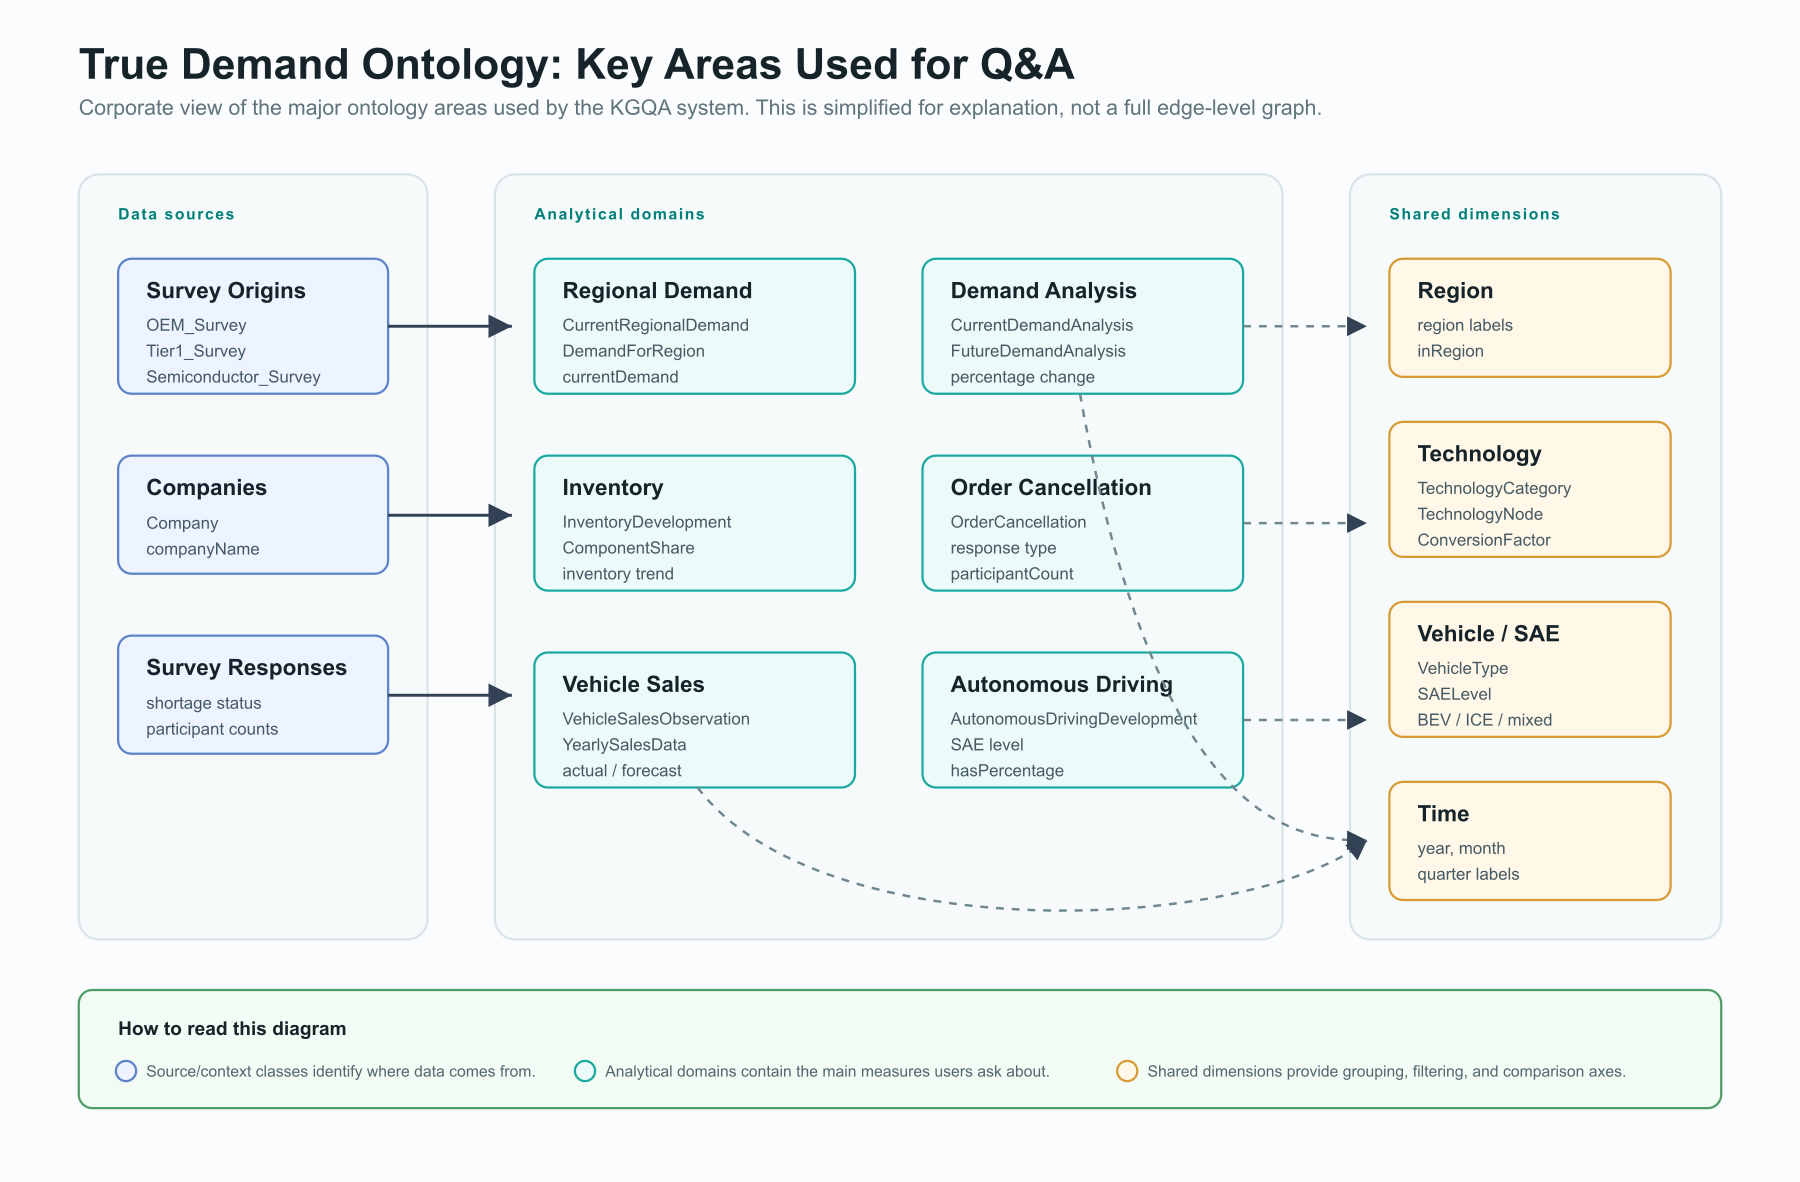
\includegraphics[width=0.95\textwidth]{docs/figures/true_demand_ontology_relationships.png}
\caption{Main ontology areas used by the True Demand KGQA system.}
\label{fig:true-demand-ontology-areas}
\end{figure}

\section{Ontology and Schema}
\label{sec:ontology-and-schema}

It is important to distinguish between the knowledge graph and the ontology/schema layer. The \textbf{knowledge graph} contains the actual RDF triples: concrete survey records, companies, regions, months, demand observations, vehicle-sales records, shortage indicators, and other instance-level data. The \textbf{ontology/schema} describes the conceptual structure of this graph: classes, properties, relationships, and expected connections between concepts.

The KGQA system uses both layers. SPARQL execution is performed over the full RDF graph. In contrast, candidate generation, validation, ranking, autocomplete, and direct routing use a schema abstraction derived from the graph. This schema abstraction is stored in \texttt{data/infineon/schema.json} and contains:

\begin{itemize}
    \item \textbf{Classes}, such as \texttt{Company}, \texttt{Region}, \texttt{FutureDemandAnalysis}, \texttt{CurrentDemandAnalysis}, \texttt{VehicleSalesObservation}, \texttt{OrderCancellation}, and \texttt{AutonomousDrivingDevelopment}.
    \item \textbf{Object-style predicates}, such as \texttt{hasSurveyOrigin}, \texttt{inRegion}, \texttt{forTimePeriod}, \texttt{analyzesVehicleType}, \texttt{analyzesTechnologyCategory}, \texttt{hasSAELevel}, and \texttt{forComponent}.
    \item \textbf{Data properties}, such as \texttt{totalDemand}, \texttt{percentageChange}, \texttt{totalDemandPercentageChange}, \texttt{unitsSold}, \texttt{participantCount}, \texttt{companyName}, \texttt{regionName}, and \texttt{periodLabel}.
    \item \textbf{Declared relationships}, which specify how classes are connected through predicates.
\end{itemize}

\begin{table}[ht]
\centering
\caption{Distinction between schema, instance graph, and capability inventory.}
\label{tab:kg-schema-capability-layers}
\begin{tabular}{p{3.0cm}p{4.5cm}p{4.5cm}p{2.8cm}}
\hline
\textbf{Layer} & \textbf{Contains} & \textbf{Used for} & \textbf{Example} \\
\hline
Ontology / schema & Classes, predicates, relationships, and abstract graph structure & Prompt construction, schema validation, visualization, feature extraction & \texttt{FutureDemandAnalysis}, \texttt{inRegion} \\
Instance knowledge graph & Concrete survey records, observations, entities, and literal values & SPARQL execution, evidence retrieval, answer generation & A demand record with region and numeric value \\
Capability inventory & Supported metric--dimension--aggregation combinations that return graph rows & Direct routing, guided autocomplete, clarification filtering & Future demand by region; vehicle sales by month \\
\hline
\end{tabular}
\end{table}

The schema is used to constrain the LLM and reduce hallucinated query structures. For example, instead of asking the LLM to invent SPARQL over an unknown graph, the system provides canonical class and property names. This helps the model generate syntactically and structurally plausible candidates. However, schema validity is not sufficient for answer correctness. A query may use valid classes and predicates but still answer the wrong business question. For example, a question asking for a grouped regional breakdown may be incorrectly answered by a scalar count query, or a question about future demand may be confused with current demand if the candidate query selects the wrong analysis class.

For this reason, the schema is also used after candidate generation. The system extracts query-plan and answer-shape features from each candidate query, including:

\begin{itemize}
    \item whether the query uses aggregation such as \texttt{COUNT}, \texttt{SUM}, or \texttt{AVG};
    \item whether the query contains a \texttt{GROUP BY} clause when the question asks for a breakdown;
    \item whether the query selects the expected metric and dimension variables;
    \item whether the query uses the expected survey scope, such as OEM, Tier1, or Semiconductor;
    \item whether the query is a ranked query, a scalar query, a grouped table, or a list lookup.
\end{itemize}

This schema-derived representation is central to the selection problem studied in this thesis. The LLM often generates multiple valid-looking SPARQL queries. The system must then decide which candidate best matches the user intent. The ontology and schema therefore play two roles: they guide generation and provide features for downstream validation and ranking.

The extracted ontology file, \texttt{data/infineon/true\_demand\_ontology\_extracted.ttl}, is used primarily for visualization and explanation. It is smaller than the full graph because it contains the schema-level view rather than every instance-level survey record. This is why ontology visualizations such as WebVOWL show the conceptual model, not all 1.16 million RDF triples. The full graph remains the execution backend for SPARQL queries.

For the thesis, it is useful to include a small schema example to show how a natural-language question maps to the graph. For example, a question about total current demand by region can be represented as a grouped SPARQL query over \texttt{DemandForRegion}, \texttt{Region}, \texttt{hasSurveyOrigin}, and \texttt{totalDemand}. Listing~\ref{lst:example-current-demand-query} shows a simplified query pattern.

\begin{lstlisting}[caption={Example graph-supported SPARQL query pattern for current demand by region.}, label={lst:example-current-demand-query}]
SELECT ?regionName (SUM(?demand) AS ?totalDemand) WHERE {
  ?entry a survey:DemandForRegion ;
         survey:hasSurveyOrigin ?origin ;
         survey:inRegion ?region ;
         survey:totalDemand ?demand .
  ?region survey:regionName ?regionName .
}
GROUP BY ?regionName
ORDER BY ?regionName
\end{lstlisting}

This example illustrates the structure that the QA system must recover from the user question: the metric is \texttt{totalDemand}, the analytical class is \texttt{DemandForRegion}, and the grouping dimension is \texttt{Region}. Similar patterns exist for future demand, shortage counts, vehicle sales, autonomous-driving indicators, inventory, and order-cancellation responses.

\section{Benchmark and Evaluation Data}
\label{sec:benchmark-evaluation-data}

In addition to the RDF graph itself, the thesis uses curated natural-language question sets and evaluation artefacts. These artefacts serve a different purpose from the graph. The graph defines what can be queried; the benchmark data defines how the KGQA system is evaluated. This separation is important because a question-answering benchmark must test not only whether the graph contains the relevant information, but also whether the system can identify the intended graph query from a natural-language request.

The repository contains an initial curated split of True Demand KGQA examples with training, development, and test files. These examples pair natural-language questions with expected query behavior and are used to develop prompts, schema features, ranking features, and evaluation scripts. The system also uses a larger set of generated and audited questions for system-level analysis, including efficiency and manual correctness evaluation. In the evaluation chapter, these datasets are used separately depending on the metric being reported.

\begin{table}[ht]
\centering
\caption{Main data artefacts used for development and evaluation.}
\label{tab:evaluation-data-assets}
\begin{tabular}{p{4.0cm}p{2.2cm}p{7.4cm}}
\hline
\textbf{Artefact} & \textbf{Size} & \textbf{Role} \\
\hline
\texttt{graph.ttl} & 1.16M triples & Full RDF execution backend for SPARQL queries \\
\texttt{schema.json} & 58 classes & Schema abstraction for prompting, validation, ranking, and routing \\
\texttt{infineon\_train.json} & 300 questions & Initial training and development of query-selection components \\
\texttt{infineon\_dev.json} & 100 questions & Development and diagnostic evaluation \\
\texttt{infineon\_test\_final.json} & 50 questions & Initial held-out evaluation set \\
\texttt{true\_demand\_efficiency\_500.json} & 500 questions & System-level efficiency and manual accuracy audit \\
\hline
\end{tabular}
\end{table}

For the final evaluation, two types of results should be reported separately. The first is \textbf{selection accuracy}, which evaluates how well the system selects the correct query among generated candidates. This is the scientific evaluation of ambiguity-aware query selection and is measured on candidate sets where LLM-generated alternatives exist. The second is \textbf{system accuracy}, which evaluates the end-to-end system, including deterministic direct templates, LLM-generated candidates, reranking, confidence routing, and clarification. This distinction prevents direct graph-supported questions from artificially hiding the difficulty of the ambiguous selection problem, while still allowing the final system to be evaluated as an engineering artefact.

\section{Data Limitations}
\label{sec:data-limitations}

The True Demand graph provides a valuable structured representation of survey-based semiconductor supply-chain information, but it also has limitations that directly affect KGQA performance. These limitations are important because they define what the system can answer reliably and what should be routed to clarification, fallback, or rejection.

\subsection{Survey-grounded coverage}

The graph is grounded in partner survey data and derived survey transformations. This means that the graph reflects what was collected, modeled, and transformed from the survey process. It does not contain every possible business fact about semiconductor supply chains. For example, the graph may contain future-demand percentages by region or technology category, but it may not contain every possible combination of product, customer, plant, lead time, or manufacturing process. A natural-language interface must therefore distinguish between questions that are answerable from the graph and questions that sound plausible but are not supported by the available data.

\subsection{Uneven class distribution}

The graph is highly uneven. Vehicle-sales observations dominate the instance-level graph, while several analytical areas contain much fewer records. This does not mean that the smaller areas are unimportant. Rather, they represent more aggregated survey outputs. However, this has practical consequences for query answering: some questions naturally return many rows, while others return only one or a few rows. The system therefore cannot rely only on schema terms. It must check whether a suggested query path actually returns data.

\subsection{Schema-valid does not mean semantically correct}

Many incorrect LLM-generated candidates are not syntactically invalid. They may use valid classes, valid predicates, and valid SPARQL syntax, but still answer a different question. For example:

\begin{itemize}
    \item a grouped breakdown may be replaced by a scalar count;
    \item a current-demand question may be answered using future-demand classes;
    \item a question asking for all groups may be answered by a ranked top-one query;
    \item a survey-specific question may omit the required survey origin;
    \item an answerable-looking query may return zero rows because the specific graph path does not exist.
\end{itemize}

This limitation is central to the thesis. It motivates the use of ML-based query selection, confidence routing, execution-aware validation, and graph-supported direct templates. The goal is not only to generate valid SPARQL, but to select a query that matches the intended business interpretation and returns graph-backed evidence.

\subsection{Limited natural-language definitions}

The ontology layer contains class and relationship structure, but it does not always contain rich human-readable definitions for every class, metric, or business concept. For instance, a class such as \texttt{Company} may exist as a schema element, but the graph may not contain a detailed textual definition explaining what counts as a company in the business context. This limits the system's ability to answer definition-style questions purely from the graph. In such cases, a production system would need either curated definitions, links to documentation such as the Digital Reference, or a controlled fallback mechanism.

\subsection{Concrete examples of graph constraints}
\label{subsec:concrete-graph-constraints}

Several limitations only become visible when natural-language questions are executed against the graph. These examples are useful because they show why the system cannot rely only on the ontology labels:

\begin{itemize}
    \item \textbf{Time granularity is domain-specific.} Vehicle-sales observations support month-level questions, but future-demand and current-demand survey outputs are not necessarily available at the same monthly granularity. Therefore, ``vehicle sales by month'' can be graph-supported while ``future demand by month'' may not be.
    \item \textbf{Survey scope changes the meaning of a query.} Demand, shortage, inventory, and autonomous-driving records may be associated with different survey origins such as OEM, Tier1, or Semiconductor. Omitting this scope can lead to a broader or different interpretation than the user intended.
    \item \textbf{Breakdown and ranking are different answer shapes.} A question phrased as ``by region'' or ``by vehicle type'' normally asks for a grouped table. It should not be automatically converted into ``which region is highest'' unless the user explicitly asks for a top, maximum, or highest value.
    \item \textbf{Catalog entities do not guarantee analytical support.} A region, technology category, or vehicle type may exist in the graph catalog, but not every metric is connected to every catalog value through a non-empty analytical path.
    \item \textbf{Counts can be misleading if the user asks for a metric.} A count of records may be valid SPARQL, but it is not the same as a total demand value, average percentage, or grouped business metric.
\end{itemize}

These examples motivated the final design of answerable autocomplete and capability-guided direct templates. The guiding principle is that user-facing suggestions should represent answerable graph paths, not merely possible ontology terms.

\subsection{Implications for the KGQA system}

These data limitations shaped several design decisions in the final system:

\begin{itemize}
    \item \textbf{Graph-supported autocomplete and guided examples}: suggested terms and generated questions should be backed by query paths that return rows.
    \item \textbf{Direct deterministic templates}: frequent graph-supported question patterns can be answered without calling the LLM.
    \item \textbf{Execution-aware selection}: candidate queries that return no rows or violate the requested answer shape should be penalized or avoided.
    \item \textbf{Clarification}: when multiple plausible interpretations remain, the system should ask the user to choose rather than force an unreliable answer.
    \item \textbf{Separation of metrics}: selection accuracy, system accuracy, coverage, and LLM cost must be reported separately because direct graph-supported questions and LLM-needed ambiguous questions have different difficulty levels.
\end{itemize}

Table~\ref{tab:data-limitations} summarizes the main limitations and their system-level consequences.

\begin{table}[ht]
\centering
\caption{Data limitations and their implications for the KGQA system.}
\label{tab:data-limitations}
\begin{tabular}{p{4.2cm}p{5.2cm}p{4.2cm}}
\hline
\textbf{Limitation} & \textbf{Effect} & \textbf{System response} \\
\hline
Survey-grounded coverage & Not every business question is answerable from the graph & Capability inventory and graph-supported suggestions \\
Uneven class distribution & Some domains return many rows, others only few & Execution checks and row-aware guidance \\
Schema-valid but semantically wrong candidates & Valid SPARQL can still answer the wrong question & ML reranking and answer-shape features \\
Missing combinations of dimensions & Some plausible breakdowns return zero rows & Direct templates only for supported paths \\
Limited textual definitions & Definition questions may lack graph evidence & Curated fallback or documentation links needed \\
\hline
\end{tabular}
\end{table}

Overall, the True Demand graph provides a realistic and challenging foundation for LLM-based KGQA. It is large enough to require structured querying, rich enough to support multiple analytical domains, and complex enough to expose ambiguity in query selection. At the same time, its survey-grounded and uneven nature makes it necessary to combine LLM generation with deterministic graph validation, ML-based selection, and user-facing clarification.
